%
% File: chap01.tex
% Author: Victor F. Brena-Medina
% Description: Introduction chapter where the biology goes.
%
\let\textcircled=\pgftextcircled
\chapter{Introduction}
\label{chap:intro}

\initial{T}he exponential growth of Information and Communication Technologies (ICTs) has played a great role in the development of tourism industry. Electronic tourism (e-tourism) is the application of ICTs for tourism purposes, including the digitalization of all its processes and value chains \cite{buhalis2003etourism}. Increasingly, ICTs provide users with access to many sources of information and has eventually affected the consumer behavior in tourism industry \cite{mills2004handbook}. Nowadays there is a huge variety of web services which provide a great complexity and diversity of recommended offers for meeting the demands of travelers. However, the personalized consumption patterns and individualistic lifestyles make it incredibly difficult for the service providers to anticipate tourists' behavior \cite{niemann2008enhancing}. Among other factors that influence the consumer behavior, trust in e-tourism is a particular challenge considering the fact that trades are geographically dispread, executed sequentially and  typically anonymous \cite{owen2014trust}. To incentivize trustworthiness, online markets employ feedback mechanisms, which allow consumers to share opinions about past experiences. Online feedback mechanisms, also known as reputation systems, \textit{have emerged as a viable mechanism for fostering cooperation among strangers in such settings} \cite{dellarocas2003digitization}. Examples of these systems, for instance TripAdvisor, Booking.com or AirBnb, after each trade encourage both parties to give feedback about their trading partner based on their own experience. 

Travelers, making use of the ICT tools that facilitate the information retrieval and decision making processes, have now direct access to all types of information provided by tourism agencies, companies, marketers, enterprises or other users. Thus, the new knowledgeable and sophisticated e-tourists  search for relevant and trustworthy information themselves instead of relying on other parties \cite{morrisonn2001predicting}. Furthermore, ICTs and Internet have transformed e-tourism markets from customer-centric to customer-driven \cite{buhalis2011tourism}, meaning that users play a major role in creating and sharing traveling information through blogs and review websites. Buhalis \cite{buhalis2011tourism} suggests that the tourism industry is now required to treat the consumers as "co-producers" of product information, considering that consumer generated content is more likely to be trusted compared to suppliers \cite{nielsen2009}. 

For online marketplaces to succeed and offer accurate information, their feedback technologies must be able to not only collect users feedback, but to properly analyze it and differentiate among sellers. The most common types of consumer generated feedback are ratings and text comments.  An important separation exists between the distinct role of text comments as tacit knowledge and ratings as explicit knowledge. According to \cite{pavlou2006nature}, text comments are particularly interesting for the audience as a new trust-building means in online marketplaces by revealing hidden knowledge that cannot be described by negative/positive ratings. In addition, consumers' needs are considered multi-dimensional and difficult to measure on discrete scales \cite{luo2005information}, therefore a traveler has to extract the needed information from different sources and types of information provided by agencies, companies or other users. This means that a big part of the work in the decision making process is totally up to the consumer. A survey by \cite{pavlou2006institutional} asked the respondents to indicate how many feedback comments they examined before each online transaction. The result showed that 81\% reported examining 25 comments (one webpage), 5\% viewed 50 comments, 11\% more than 50 ones, and only 3\% did not examine any text comments. These findings reveal that despite the importance of text feedback to the users, it is difficult for them to access the meaning of numerous text comments \cite{pavlou2006institutional}.  Given this situation, the average human reader will have difficulties on identifying and extracting the relevant information from the opinions in them.  

Current online travel systems, aiming to assist the consumer in finding suitable offers, allow the user to rank and filter the information based on location-price factor or on the overall ratings accumulated from the feedback system. However, this does not necessarily mean that the top result is the most suitable for a certain user considering the personal requirements. For example, let us consider a person who has trouble sleeping and therefore  a \textit{quiet} place is a non-negotiable personal requirement. A room in the city center, with a very good price and high rating may not be suitable because it may be also \textit{noisy}. The customer in this case would have to check all the text comments of each listing in the search results in order to find the proper match. This task is not only time consuming but also inefficient, given that most of the users will not read all the reviews and may end up picking something random. 

The service providers often offer summaries to all feedback comments, which mostly consist on a bunch of most used words. However, this bag of words does not necessarily cover the features that a certain user is interested in. In cases when the list contains the feature, it provides no other information except of the fact that it is mentioned somewhere in the comments. The user still has to read for each listing all the text comments related to the feature, meaning that it still does not reduce much of the travelers' work. Automated analysis systems are thus needed \cite{liu2012sentiment}. Natural language processing (NLP) enables computers to derive meaning from any human written input, including their opinions. The NLP methods for doing so fall into the category of sentiment mining methods, known also as \textit{opinion mining}. 

This paper proposes a pipeline, which uses an ontology based approach combined with sentiment mining techniques for generating opinion scores for each accommodation feature mentioned in the reviews of a feedback system. The sentiment score serves in this case as a discrete estimator of the customer requirements, which are represented by accommodation features. This pipeline aims to offer to the users the possibility of ranking the accommodation search results based on their "difficult to measure" individualistic requirement, besides the price-location ranking factors. The research itself aims to give an answer to the following two questions. Firstly, \textit{how good can feature-based opinion mining estimate the quality of customer requirements represented by accommodation features in e-tourism feedback systems?} Secondly, \textit{how will the implementation of this pipeline in the search systems affect the customer satisfaction during the decision making process?} To provide an answer to these two questions this paper is organized as follows. The first part of the paper introduces the importance of gathering and analyzing customer information and requirements in e-tourism as treated by the Customer Focus theory. Then it provides a short introduction to the online feedback systems, as important tools for gathering customer information, including the characteristics of the most popular travel web services and the methods they use for analyzing customer reviews. The current state-of-the-art of feature-based opinion mining used for analyzing customer feedback is covered in the second part. Further, the proposed approach is discussed, consisting explanation of the pipeline step by step. The fourth chapter covers the methodology used for this research, which leads to the results presented in chapter five. Lastly the paper evaluates the proposed approach and ends up with the practical implications of this work, limitations and further work to be done. 

\section{Customer Focus Theory}
\label{sec:CFTH}

When offering a service or product, it is essential to understand what consumers' preferences are and how can we shape the offerings accordingly to create value. Customer Focus Theory is one of Information Studies theories, which specifically offers a guide on how to put the focus on the customer. This theory should be explained according to the context of my research (where it is placed and adds value on the framework) as shown in Figure \ref{fig:CustomerFocus}. 
--- Narrow down to "Receiving and utilization of customer feedback" and the accordance with the research topic.

--- Check \cite{lohan2011examining} and change thesis focus to customer oriented!! 


\label{sec:OFS}
\begin{figure}[h!]
	\centering
	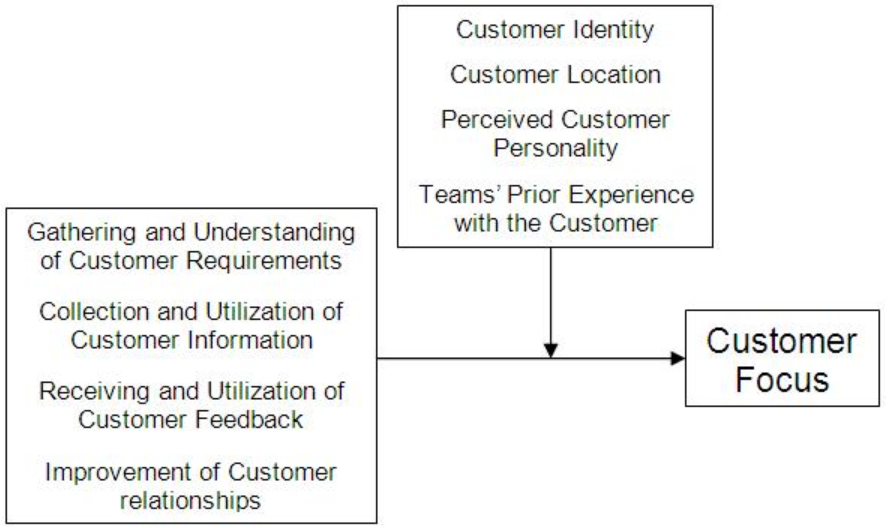
\includegraphics[height=0.3\textheight]{fig01/CustomerFocus}
	\caption{Theoretical framework of Customer Focus theory}
	\label{fig:CustomerFocus}
\end{figure}

\section{Online Feedback systems}
%Methods for analyzing customer feedback

This section will explain how online feedback systems work. It will describe, categorize and point out the differences between the typical types of OFS used by the most successful online marketers (TripAdvisor, Booking.com, Airbnb, couchsurfing etc). 